
\documentclass[11pt,a4paper]{article}
\usepackage{times}
\usepackage{latexsym}
\usepackage[nohyperref]{nlp_project}

\usepackage{url}
% allows for temporary adjustment of side margins
\usepackage{chngpage}
\usepackage{graphicx}
\graphicspath{ {./images/} }


\aclfinalcopy


\title{Textual analysis of security filings for long-term stock price prediction }

\author{ NLP Course - Open U: 2019 \\
  Tomer Rothschild \\
  ID:034702076 \\
  \texttt{rotomer9@gmail.com} }

\date{}

\begin{document}
\maketitle
\begin{abstract}
  I explore the predictability of long-term stock price changes using text analysis. In particular, I show that adding features using NLP techniques from multiple layers of linguistic analysis yields superior long-term prediction power over quantitative, financially-rooted models.
\end{abstract}

\section{Introduction}
Algorithmic trading, and automatic analysis of information related to stocks has been applied at massive scale. Most of the existing approaches are focused on predicting short-term swings in stock prices. Thus, these approaches are mostly used by companies with the resources to compete on the grounds of split-second processing, while making the transaction costs negligible via the sheer scale of each transaction.

This situation had gradually pushed individual investors out of the stock market as they couldn't compete on the same grounds as the corporates because the resources needed for that are out of reach of the individual investor. However, as corporates' performance is often measured on a quarterly basis, corporates face temporal constraints which do not affect the individual investors. Moreover, with long term trades the effect of the trading transaction costs diminishes greatly as they make a smaller percentage of a potentially much bigger price change (without mandating large-scale transactions). This makes long term-stock price prediction especially relevant for the individual investor.

I present a system for textual analysis of security filings, and a long-term price trend predictor based on the textual analysis. The contributions of my work are:
\begin{itemize}
  \item I demonstrate that the textual part of the 8-K and 10-K financial reports, which must be filed by publicly listed U.S. companies, carries information which correlates with the corresponding company's stock long-term performance (over 2 years). I also show that this extra information is not generally available through other financially-rooted means.
  \item I implement a model that predicts the trend of stocks over a series of time periods using features that were extracted from the textual analysis, as well as financially-rooted features like analyst earnings surprise.
  \item I show that the model which includes textual based features performs significantly better over the long term than a model with just quantitative, financially-rooted features.
\end{itemize}
 

\section{Related Work}
\subsection{Prior Art}

Various methods incorporating natural language processing and machine learning algorithms to predict stock prices have been explored in prior art.

Cohen et al. (2018) \cite{cohen2018lazy} have found that stock price changes correlate with the degree of change in the textual parts of 10-K security filings. Lee et al. (2014) \cite{lee2014importance} have shown that using textual analysis of 8-K security filings may increase the prediction power of stock prices for the short term (up to 5 days). 

Loughran et al. (2011) \cite{loughran2011liability} have suggested that the widely used Harvard dictionary has limited applicability when analyzing the tone of security filings, and have published an alternative dictionary.

Engelberg (2008) \cite{engelberg2008costly} shows that linguistic information, perhaps because of cognitive load in processing, has greater long-term predictability for asset prices than quantitative information. It is important to mention that Lee et al. (2014) didn't manage to repeat Engelberg's result in terms of long-term predictability, whereas the method shown in this paper yields superior long-term predictability using textual analysis (over using just quantitative information).

Ball et al. (1968) \cite{ball1968empirical} find that companies with actual earnings that exceed or fall short of earnings estimates experience abnormal returns over subsequent periods. I use this finding as the quantitative, financially-rooted baseline-feature in the prediction.

\subsection{Related Methods}
I have used the following algorithms \& libraries as part of this paper (this will be further explained in the next section - Methods and Model):
\begin{enumerate}
  \item Relation extraction using open domain information extraction (Open IE) in Stanford CoreNLP (Java) library. Based on Angeli et al. (2015) \cite{angeli2015leveraging}
  \item Tokenization, Lemmatization \& POS-tagging using NLTK \cite{loper2002nltk}.
  \item Specialized text tone extraction using the dictionary published by Loughran et al. (2011).
  \item Sentiment analysis using TextBlob \& Pattern \cite{smedt2012pattern}.
  \item Cosine similarity using Scikit-learn \cite{pedregosa2011scikit}.
  \item Gradient-boosted random-forest classifier using Scikit-learn.  
  \item McNemar significance test using StatsModels \cite{seabold2010statsmodels}
\end{enumerate}

\section{Method and Model}

The method used in this paper is composed of two main parts:
\begin{itemize}
  \item Feature extraction (see sub-sections below).
  \item Price trend classification using a gradient-boosted random-forest classifier.
\end{itemize}

\subsection{Baseline features}
I use quantitative, financially-rooted features as a baseline. This baseline enables the attribution of a measurable amount of added prediction-accuracy to the features extracted via textual analysis. The approach I have taken in this paper is based on the baseline that was used in Lee et al. (2014) - which is to use analyst consensus on stock earning-per-share surprise (EPS). This single quantitative feature contains a wealth of information  - it expresses the ratio between the market expectations and the actual performance of the underlying company. 

In addition to the EPS-surprise feature, which is published quarterly, I have added a second feature to the baseline - time-since-EPS. This feature expresses the number of days since the last EPS surprise was published. Tracking the number of days between the publish-date of the security filing which text is analyzed is important for the predictor to determine the relative weight of the EPS-surprise factor.

\subsection{Features engineered via Relation Extraction}
Open domain information extraction is used in order to extract relation triples in the form of: (Subject, Relation, Object). As mentioned earlier, this is performed using OpenIE in the Java library Stanford CoreNLP. The algorithm which is applied uses dependency parsed structure of a sentence in order to infer relevant relations between subject and object across clauses, as well as within clauses.

I've chosen to use open IE relation extraction because I had no corpus of security filings tagged with relations - which made other approaches like distant supervision less tractable (especially given the different jargon/dictionary used in security filings).

The extracted relations are used to infer whether the CEO or CFO of the company have been reported to be leaving the company.

\subsection{Features engineered via similarity metrics}
Pairwise cosine similarity index is used in order to measure the difference between consecutive filings. \\
The pipeline applied in order to compute the pairwise cosine index of two texts is as follows:
\begin{enumerate}
  \item The texts are tokenized (using NLTK).
  \item Each token is POS tagged (using NLTK).
  \item Each token is transformed into its lemmatized form (using NLTK, aided by the POS tagging of each token to improve the lemmatization). 
  \item The lemmatized texts are then vectorized by count per lemmatized token.
  \item The cosine similarity is computed on the vectors according to the following formula:
  \[ cosine\_sim(A,B) = \frac{A \cdot B}{||A|| \cdot ||B||} = \]
  \[ = \frac{\sum_{i=1}^{n} A_i B_i}{\sqrt{\sum_{i=1}^{n} A_i^2} \cdot \sqrt{\sum_{i=1}^{n} B_i^2}} \]
  Where $A_i, B_i$ are components of vectors A \& B respectively.
\end{enumerate}
\\
The rationale behind adding this feature is based on the observation made by Cohen et al. (2018) that stock price changes correlate with the degree of change in the textual parts of security filings.

\subsection{Features engineered via specialized tone extraction}
A special dictionary is used to extract several tone features. These features are extracted using a specialized dictionary for texts in financial statement and security filings.

The model for the extraction is a unigram model in which we count the occurrences of words within each of the categories. \\
The extracted tone dimensions are: Positive, Negative, Uncertainty, Litigious, Constraining, Superfluous, Interesting \& Modal.


\subsection{Features engineered via sentiment analysis}
Sentiment polarity \& subjectivity metrics has been computed for each of the texts of the filings using the TextBlob library.

\subsection{Features engineered via exponential smoothing}
Given the time-series nature of stock price prediction, I've also introduced exponential-average feature counterparts for each of the textual features.
The exponential-average is defined as follows:
\[ s_0 = x_0 \]
\[\ s_t = \alpha x_t + (1-\alpha)s_{t-1} , t > 0\]
Where $ x_t $ denotes the raw data at time $t$, and the output of the exponential-smoothing algorithm is denoted by $ s_t $. \\
Generally, $\alpha$ - the "smoothing factor" - maintains: $0 < \alpha < 1$. The $\alpha$ value being used for this feature is $0.5$.
  
\section{Data}
The algorithm uses the following data sets:
\begin{enumerate}
  \item \textbf{8-K corpus} \\
8-K security filings must be filed by publicly listed U.S. companies when major events occur which may impact the stock price of the corresponding company.

The source of the 8-K filings is from the data that was published by Lee et al. (2014). This data is already a processed version of the complete 8-K forms. The processing that was already done is removal of html tags, and removal of tables with numeric values. The resulting format is therefore plain text files. I have processed the data from Lee et al. (2014) further and indexed it such that it can be accessed easily by the algorithm's feature extraction steps.

The corpus covers all of the 8-K filings for the companies listed on the S\&P 500 index during the years 2002-2012. The size of the corpus is 2.3 GB.

  \item \textbf{10-K corpus} \\
  10-K is the annual report that must be filed by publicly listed U.S. companies. This filing is aimed to give a comprehensive summary of a company's financial performance.
  
  The source of the 10-K corpus is from EDGAR. EDGAR is the Electronic Data Gathering, Analysis, and Retrieval system used at the U.S. Securities and Exchange Commission (SEC). I have scraped the EDGAR system for the required corpus of 10-K files.
  
  I have performed pre-processing on the 10-K forms and extracted just a single section for further textual analysis and feature extraction. The chosen section is "Managements Discussion and Analysis of Financial Condition and Results of Operations" (MD\&A). The MD\&A section is a free-form section in which the management provides commentary on financial statements, systems and controls, compliance with laws and regulations, and actions it has planned or has taken to address any challenges the company is facing.
  
  The corpus covers all of the 10-K filings for the companies listed on the S\&P 500 index during the years 2002-2012. The size of the corpus is 712 MB.
  
  \item \textbf{Earning-per-share surprise} \\
Earning-per-share (EPS) surprise is the gap between consensus and reported EPS. Consensus EPS is the analysts’ estimation of earnings per share, and reported EPS is the actual earnings
per share as reported by the company.

The source of this data set is from Lee et al. (2014).

This data set covers companies listed on the S\&P 500 index during the years 2002-2012.
  \item \textbf{Daily stock prices} \\ 
The daily stock prices data set has the target values of our prediction. 

The source of this data set is from Lee et al. (2014). In order to be used as the target of the final classification model, I have processed the daily price data to binary labels (UP / DOWN) which denote the price trend of a given stock at a given time-window.

This data set covers companies listed on the S\&P 500 index during the years 2002-2012.
\end{enumerate}
\section{Experiments}
For the experiments I have split the data by companies with a ratio of 80/20 for train/test respectively. The hyper parameters of the prediction model were determined for the training-set using a randomized search 10-fold cross validation.

I compare my system against a simple but
very strong baseline which is based on the EPS features. Lee et al. (2014) have found that the earnings surprise
feature is the single most important feature in their feature set.

To see how the event of an 8-K / 10-K filing influences the company's stock price over time, I calculate the price change, which is used to generate the UP / DOWN label, at various time-frame "horizons": 5 days, 30 days, 90 days, 180 days, 360 days, 720 days \& 1,080 days.

For each of the corpora we train an independent predictor. In other words, two different predictors are trained for each of the time-frame horizon experiments (the two predictors are: one for the 8-K corpus, and one for the 10-K corpus). During the prediction phase - the appropriate predictor is chosen depending on the type of the event (8-K / 10-K).

\subsection{Experimental results}
As we can see, from Tables 1. \& 2. and Figures 1. \& 2. - the baseline feature EPS surprise is very informative for this task. Moreover, both the baseline prediction and the linguistic-features-enhanced-prediction provide higher accuracy the longer the time-frame horizon of the prediction. Interestingly, this seems to come at the cost diminishing F1 scores.

It is also apparent that the linguistic-features-enhanced -prediction provides superior results for long-term predictions. 
\begin{table}[h!]
\begin{tabular}{ |p{1.4cm}| p{1.5cm} p{1.2cm} c c|  }
 \hline
 \multicolumn{5}{|c|}{8-K Prediction Results} \\
 \hline
 Time-frame Horizon (in days)& Baseline Accuracy & Accuracy & Baseline F1 & F1\\
 \hline
5    & 0.5335 & 0.5378 & 0.6230 & 0.6294\\
30   & 0.5670 & 0.5671 & 0.6986 & 0.6935\\
90   & 0.5963 & 0.5933 & 0.7222 & 0.7061\\
180  & 0.6061 & 0.6145 & 0.7245 & 0.7090\\
360  & 0.6186 & 0.6288 & 0.7077 & 0.6933\\
720  & 0.6298 & 0.6469 & 0.6471 & 0.6636\\
1080 & 0.6378 & 0.6499 & 0.6092 & 0.6356\\
 \hline
\end{tabular}
\caption{Comparison of prediction results using the 8-K corpus between the baseline prediction and the prediction enhanced with linguistic features}
\label{table:1}
\end{table}

\begin{table}[h!]
\begin{adjustwidth}{0in}{0in}
\begin{tabular}{ |p{1.4cm}| p{1.5cm} p{1.2cm} c c|  }
 \hline
 \multicolumn{5}{|c|}{10-K Prediction Results} \\
 \hline
 Time-frame Horizon (in days)& Baseline Accuracy & Accuracy & Baseline F1 & F1\\
 \hline
5    & 0.5437 & 0.5431 & 0.6405 & 0.6456\\
30   & 0.5656 & 0.5568 & 0.6965 & 0.6888\\
90   & 0.5955 & 0.5962 & 0.7173 & 0.6993\\
180  & 0.6075 & 0.6142 & 0.7232 & 0.7030\\
360  & 0.6166 & 0.6189 & 0.7046 & 0.6833\\
720  & 0.6240 & 0.6319 & 0.6235 & 0.6342\\
1080 & 0.6265 & 0.6381 & 0.5606 & 0.5872\\
 \hline
\end{tabular}

\caption{Comparison of prediction results using the 10-K corpus between the baseline prediction and the prediction enhanced with linguistic features}
\end{adjustwidth}
\label{table:2}
\end{table}

\begin{figure}[t]
\begin{adjustwidth}{-0.5in}{0in}
\caption{}
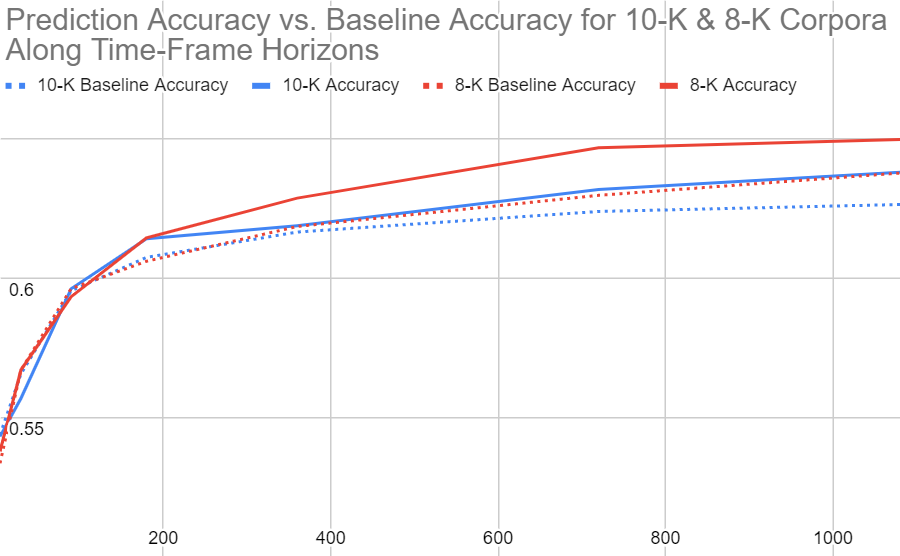
\includegraphics[scale=0.285]{accuracy_figure}
\end{adjustwidth}
\end{figure}

\begin{figure}[h]
\begin{adjustwidth}{-0.5in}{0in}
\caption{}
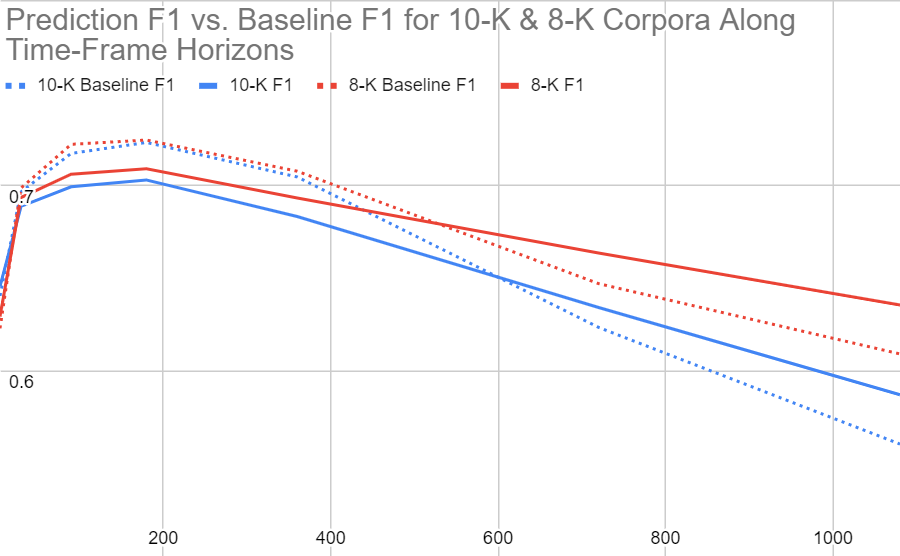
\includegraphics[scale=0.275]{f1_figure}
\end{adjustwidth}
\end{figure}

\section{Evaluation}

Table 4. shows the how significant is the difference between the two models: the baseline and the linguistic model. The significance of the difference is computed using the McNemar test via the StatsModels library \cite{seabold2010statsmodels} 

We compute a contingency matrix of the form:
\begin{table}[h!]
\begin{adjustwidth}{0in}{0in}
\begin{tabular}{ |p{2cm}| p{2cm} | p{2cm}|  }
 \hline
 & Classifier 2 correct & Classifier 2 incorrect\\
 \hline
Classifier 1 correct   & Yes / Yes & Yes / No\\
\hline
Classifier 1 incorrect & No / Yes  & No / No \\
 \hline
\end{tabular}
\caption{Contingency table}
\end{adjustwidth}
\label{table:3}
\end{table}


Given the contingency matrix, the McNemar statistic is defined as:
\[ statistic = \frac{(Yes/No - No/Yes)^2}{Yes/No + No/Yes} \]


\begin{table}[h!]
\begin{adjustwidth}{0in}{0in}
\begin{tabular}{ |p{2cm}| p{2.5cm} p{2.5cm}|  }
 \hline
 Time-frame Horizon (in days)& 8-K McNemar p-value & 10-K McNemar p-value\\
 \hline
5    & 0.417 & 0.918\\
30   & 1.000 & 0.016\\ % here 10-K is significantly worse
90   & 0.531 & 0.916\\
180  & 0.127 & 0.250\\
360  & 0.105 & 0.727\\
720  & 0.006 & 0.095\\
1080 & 0.032 & 0.036\\
 \hline
\end{tabular}

\caption{Significance of the difference between the prediction results using the 10-K corpus between the baseline model and the model enhanced with linguistic features}
\end{adjustwidth}
\label{table:4}
\end{table}

We can see in Table 4. that with $\alpha$-value = 0.05, then the model with linguistic features is significantly better in the long-range of 3-years for both of the corpora. While the model for the 8-K corpus has been shown to pass the significance criteria for the 2-years time-range as well, the level of improvement for the model for the 10-K corpus over the baseline for this time-range is borderline to be proven significant.

As can also be observed from the figures,  there's hardly any difference between the model with linguistic features and the baseline model during the short time-ranges (aside from what seems to be an outlier where the baseline outperforms the linguistic model significantly for the 10-K corpus in the 30-day time-range).

\section{Discussion}

The results from the time-frame horizon experiments, as well as the evaluations for significance of the results lend some interesting insights. 

As mentioned above, once we move past the first two years from the filing date \& EPS surprise date - we can observe that the signal from the linguistic features provides additional information when compared to the baseline model. This suggests that the model can indeed be used as an aid for long-term investment as it improves upon the prediction which represents the generally available data.

A possible explanation for the results of this paper is that linguistic analysis of security filings uncovers fundamental attributes of company behaviour that take years to manifest, and have a definitive role in the long-term trend of the price of stock.   

Regardless of the underlying cause, these results are an improvement in terms of applicability for the individual investor for which long-term investment is the ground at which he is not at a disadvantage with the corporates. The improvement mentioned here relates to the limitations stated in Lee et al (2014).

\section{Conclusion}
In this work, I have presented a textual analysis model that was provides superior long-term prediction power over a financially rooted baseline model. The proposed model is of particular potential applicability for the individual investors, but further analysis needs to be done before it can be used as a trading tool (for example, risk derived from the stocks preferred by the model has not been considered as part of this work).

\section{Suggestions for Future Work}
Further linguistic analysis of security filings and other textual resources may improve upon the results of this paper. A few possible directions for further analysis are:
\begin{enumerate}
  \item Engineering of additional features from relation extraction.
  \item Using additional features from textual analysis from other linguistic layers. Note that Lee et al. (2014) had negative results using bigram models and dependency-based features.
  \item Analyzing 10-Q security filings as well. 10-Q filings are a shortened version of the 10-K form and are filed quarterly by most of the companies (as opposed to 10-K which is filed annually by all companies).
  \item Analyzing the risk derived from the stocks preferred by the model as measured by past volatility, and factoring this consideration into the model to reduce the induced trading risk.
\end{enumerate}

\section{Additional Resources}
Repositories:
\begin{enumerate}
  \item Main project repository - https://github.com/rotomer/nlp-project
  \item Stanford CoreNLP wrapper repository (the standard open source python wrapper for Stanford CoreNLP failed to cope with large processing relation extractions of large files - so I've created my own wrapper that performed the main IO with files rather than over HTTP) - https://github.com/rotomer/stanford-corenlp-wrapper 
\end{enumerate}

\section{Bibliography}
\bibliographystyle{plain}
\bibliography{refs} 

\end{document}
